%% DESIGN: Noto Sans | Growth-showing, progression-visible | Navy (#1A237E) accent
\documentclass[11pt,a4paper]{article}
\usepackage[left=0.6in,right=0.6in,top=0.5in,bottom=0.5in]{geometry}
\usepackage[T1]{fontenc}
\usepackage[sfdefault]{noto-sans}
\usepackage{xcolor,titlesec,enumitem,hyperref,tikz}

\definecolor{accent}{HTML}{1A237E}
\definecolor{ACCENT}{HTML}{1A237E}
\definecolor{lightaccent}{HTML}{E8EAF6}
\hypersetup{colorlinks=true,urlcolor=accent}
\pagestyle{empty}

\titleformat{\section}{\large\bfseries\color{accent}}{}{0em}{}[\vspace{-0.5em}\textcolor{accent}{\rule{\linewidth}{1.5pt}}]
\titlespacing{\section}{0pt}{1em}{0.4em}

% Progression arrow
\newcommand{\progression}{\textcolor{accent}{$\longrightarrow$}}

\begin{document}

% Header with progression indicator
\noindent

\begin{tikzpicture}
\fill[accent] (0,0) rectangle (\textwidth,2.2);
% Growth arrow
\draw[white,ultra thick,->] (0.5,0.3) -- (\textwidth-0.5,0.3);
\foreach \x/\lab in {1/Junior, 5/Mid-Level, 9/Senior, 13/Next} {
  \fill[white] (\x,0.3) circle (4pt);
  \node[white,font=\tiny,above] at (\x,0.5) {\lab};
}
\node[anchor=west,text=white,font=\Huge\bfseries] at (0.3,1.5) {MARCUS CHEN};
\node[anchor=east,text=white!90,font=\large] at (\textwidth-0.3,1.5) {Software Development Engineer};
\node[anchor=east,text=white!75,font=\small] at (\textwidth-0.3,0.9) {marcus.chen@email.com | (555) 234-5678 | Seattle, WA};
\end{tikzpicture}

\vspace{0.5em}

\section{Summary}
Mid-level Software Engineer with 4 years of progressive growth from junior developer to technical lead on key projects. Full-stack expertise with a backend focus. Seeking senior roles where I can own system design and mentor others.

\section{Career Progression}

% Current role - emphasized
\noindent
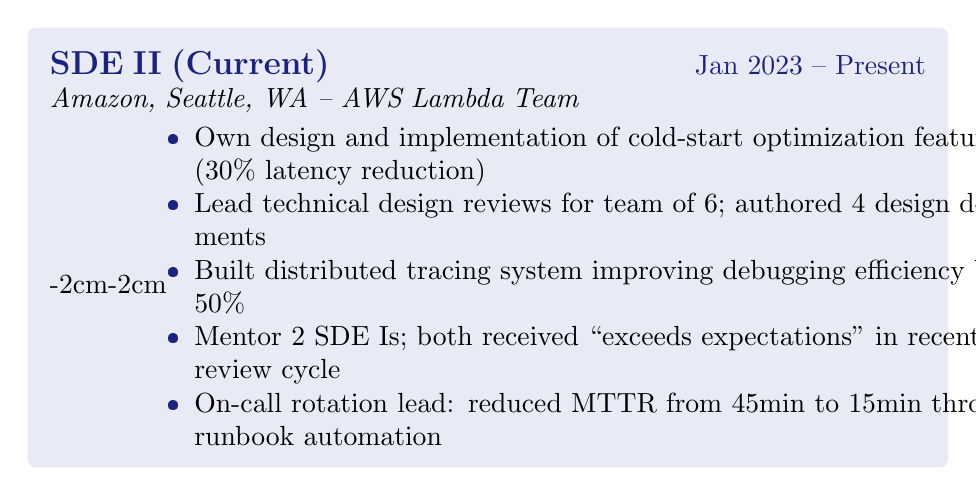
\begin{tikzpicture}
\node[fill=lightaccent,rounded corners=3pt,inner sep=8pt,text width=\textwidth-1cm] {
\textbf{\large\color{accent} SDE II (Current)} \hfill \textcolor{accent}{Jan 2023 -- Present}\\
\textit{Amazon, Seattle, WA -- AWS Lambda Team}\\[4pt]
\begin{minipage}{\textwidth-2cm}
\begin{itemize}[leftmargin=1em,nosep,label={\color{accent}\textbullet}]
\item Own design and implementation of cold-start optimization feature (30\% latency reduction)
\item Lead technical design reviews for team of 6; authored 4 design documents
\item Built distributed tracing system improving debugging efficiency by 50\%
\item Mentor 2 SDE Is; both received ``exceeds expectations'' in recent review cycle
\item On-call rotation lead: reduced MTTR from 45min to 15min through runbook automation
\end{itemize}
\end{minipage}
};
\end{tikzpicture}

\vspace{0.5em}

\noindent\textbf{SDE I} \hfill \textcolor{accent}{Jun 2021 -- Dec 2022}\\
\textit{Amazon, Seattle, WA -- AWS Lambda Team}
\begin{itemize}[leftmargin=1.2em,nosep,label={\color{accent}\textbullet}]
\item Delivered 3 major features for Lambda runtime, serving millions of invocations daily
\item Reduced deployment pipeline time by 40\% through parallelization and caching
\item Promoted to SDE II in 18 months (typical: 24 months) based on scope and impact
\item Received ``Exceeds'' rating in all review cycles
\end{itemize}
\vspace{0.5em}

\noindent\textbf{Software Engineer} \hfill \textcolor{accent}{Jul 2020 -- May 2021}\\
\textit{Startup XYZ (Series A), San Francisco, CA}
\begin{itemize}[leftmargin=1.2em,nosep,label={\color{accent}\textbullet}]
\item Built core backend services (Go) for real-time collaboration platform
\item Implemented WebSocket infrastructure supporting 10K concurrent connections
\item First engineering hire; helped grow team from 2 to 8 engineers
\end{itemize}

\section{Technical Skills}
\noindent\textbf{Languages:} Java (primary), Go, Python, TypeScript \quad\textbf{Systems:} Distributed Systems, Microservices, Event-Driven\\
\textbf{AWS:} Lambda, DynamoDB, SQS, ECS, CloudFormation \quad\textbf{Tools:} Docker, Kubernetes, Terraform, CI/CD

\section{Education}
\noindent\textbf{B.S. Computer Science} \hfill University of Washington, 2020 \quad(GPA: 3.7)

\section{Growth Indicators}
\noindent\textcolor{accent}{\textbf{Scope:}} Individual tasks \progression{} Feature ownership \progression{} System design \progression{} Cross-team influence\\
\textcolor{accent}{\textbf{Impact:}} Bug fixes \progression{} Feature delivery \progression{} Architecture decisions \progression{} Mentoring others

\end{document}
